\setcounter{chapter}{-1}
%%%%%%%%%%%%%%%%%%%%%%%%%%
\chapter{Proposal Summary}
%%%%%%%%%%%%%%%%%%%%%%%%%%

This chapter will not be part of the final thesis but serves as more of an executive summary of where I am in the thesis process.
\Cref{tab:timeline} describe the notional timeline of my doctoral work.
The following to sections briefly summarize the papers I have completed so far, and the papers that I plan to publish to complete my thesis.
More substantial descriptions of the work are given in the body of thesis.


\begin{table}
  \centering
  \begin{tabular}{lll}
  \toprule
  2019 & August & Began research master's degree (CMU) \\
  2021 & August & Completed masters, began PhD \\
  2024 & July--September & XferBench eval (\Cref{ch:xferbench-analysis}) \\
  & September & Proposal \\
  & October--December & Rich corpora (\Cref{ch:rich-corpora}) \\
  2025 & January--March & Morphemes (\Cref{ch:morphemes}) \\
  & April--June & Morpheme structure (\Cref{ch:syntax}) \\
  & July & Defense \\
  \bottomrule
  \end{tabular}

  \caption{Timeline}
  \unskip\label{tab:timeline}
\end{table}

\section{Completed Work}
% The following completed research papers will be incorporated into the thesis (either in part or their entirety).
% Other work has be published and/or completed during the course of my master's and doctoral work but will not play major role in the thesis.


\subsection{Recommendations for Systematic Research on Emergent Language}
\noindent
\citet{boldt2022recommendations} was rejected from ICML 2022; part of this work was expanded into ``A Review of the Applications of Deep Learning-Based Emergent Communication'' discussed below.
This is a position paper which critiques and makes recommendations for emergent communication research from a meta-scientific angle.
It begins by specifying the goals of emergent communication research (which would eventually become the TMLR paper).
In light of these goals, which are split between ``engineering'' and ``scientific'' goals, the paper discusses core methodological elements of engineering and science.
Finally, each of the core methodological elements is explicitly detailed in the context of emergent communication.
In addition to the goals, the particular elements of engineering which are pursued in this thesis are evaluation metrics and standard datasets.

\subsection{A Review of the Applications of Deep Learning-Based Emergent Communication}

\noindent
\citet{boldt2024review} was published in the \textit{Transactions of Machine Learning Research} (TMLR) in February 2024.
This paper comprehensively reviews the applications and goal of emergent communication research drawing on both the literature and the author's (i.e., Brendon and David's) experience in the field.
Each application, in addition to a description and review of the relevant literature, is a accompanied by a brief set of recommendations on the most fruitful next steps for that research direction.
The set of applications themselves is divided into three categories:
  (1) internal applications, which focus on improving the methods of emergent communication itself,
  (2) task-driven applications, which look at engineering tasks focused on more effectively solving particular problems,
  and (3) knowledge-driven applications, which aim at increasing scientific understanding of particular phenomena.

\subsection{XferBench: a Data-Driven Benchmark for Emergent Language}
\noindent
\citet{boldt2024xferbench} was published in the \textit{Proceedings of the 2024 Conference of the North American Chapter of the Association for Computational Linguistics: Human Language Technologies (Volume 1: Long Papers)} (NAACL).
This paper introduces a first-of-its-kind evaluation metric/benchmark for emergent languages.
It addresses the question of the \emph{quality} of an emergent language by looking at its similarity to human language from a data-driven, machine learning perspective.
Specifically, it quantifies ``similarity to human language''---and, therefore, overall quality---as how much pretraining on an emergent language corpus improves performance on modeling human language (although we also test machine translation).
XferBench is published as an easy-to-use Python package, and since it only requires an unannotated corpus of utterances from the emergent language, it is intended to have widespread use in emergent communication research.


\subsection{ELCC: the Emergent Language Corpus Collection}
Under review at the \textit{2024 Conference on Neural Information Processing Systems Datasets and Benchmarks Track} (decision in September 2024).
This paper introduces a collection of over $70$ emergent language corpora from across $8$ different systems in the literature.
Each of these corpora is annotated with statistical analyses as well as metadata documenting the features of the system/environment it came from.
Such a resource is intended to make studying emergent languages themselves far easier since it obviates the need run the systems oneself and enable comparative studies given the variety of emergent communication systems included.

\subsection{Other Work}
Some work completed during the course of master's and doctoral work will not factor heavily into the thesis.
In ``Mathematically modelling the lexicon entropy of emergent language'' \citep{boldt2022mathematically}, we investigate using a formal model based on the Chinese restaurant process to make predictions of the entropy of lexica in emergent languages; this is intended to be a sort of exemplar of using formal models to make clear, determinate hypotheses regarding emergent communication experiments.
In ``Shaped rewards bias emergent language'' \citep{boldt2022shaped}, we argue that reward shaping (a common feature of reinforcement learning experiments) has the potential to bias (i.e., predetermine) properties of the resulting emergent language.
In ``Case study: deontological ethics in NLP'' \citep{prabhumoye-etal-2021-case}, we apply deontological approach to ethics to different real-world scenarios in natural language processing-based systems.



\section{Proposed Work}
This section will briefly described the proposed work for the completion of the doctoral thesis.
Each of these papers is intended to a standard conference-length paper (i.e., 8--9 pages).

\subsection{XferBench analysis}
In this paper, which is currently in progress, we will run XferBench on all of the languages in ELCC in order to find correlations between XferBench performance and features of the corpora and emergent communication system they come from.
For example, we hope to answer question such as ``Do more complex environments yield better emergent languages?'' or ``Is token entropy of an emergent language predictive of its score on XferBench?''
These analyses will help to understand what XferBench is measuring and whether it is easily explainable by surface-level statistics of the corpus or whether some deeper structural characteristics might be required to understand XferBench's outputs.


\subsection{Rich emergent language corpora}
ELCC, the current collection of emergent language corpora, only includes the corpora themselves and aggregate statistics, but many interesting research directions require not only having access to the tokens of utterances themselves but also their context.
For example, anything related to semantics is going to require some way to determine what an utterance means.
Thus, we propose an extension to ELCC which takes the same set of corpora and includes information about the state of the environment before and after each utterance so as to supply grounding for each of the utterances.
From here, it will be possible to explore a far greater range of phenomena with respect to the emergent language corpora in ELCC\@.

\subsection{Automatically detecting morphemes in emergent language corpora}
While the original plan was to create a linguistic counterpart to XferBench, that is, some benchmark-like metric which measured the presence of human language-like linguistic structures in emergent communication, I rolled back my ambition considerably as there are not yet methods for detecting structure in emergent communication generally.
Thus, this project will make an important step in the direction of such a metric by introducing and testing an algorithm to detect and segment emergent communication utterances into morphemes: particular meanings paired with an atomic form.
Detecting morphemes is critical in building up to ``higher-level'' linguistic concepts like syntax and discourse, yet there are no existing methods determining what the meaningful units of an emergent communication utterance are in a general, system-agnostic way (e.g., is each token its own morpheme are they sub-morpheme units?).
This work will leverage the rich emergent language corpora discussed above as it is necessary to pair the utterances (form) with the accompanying context (meaning) in order to uncover morphemes (or at least an analogous structure).
Being able to turn emergent languages represented as strings of raw tokens into strings of morphemes will enable more principled research on linguistic structures which presuppose the existence and identification of morphemes (e.g., syntax).

\cmt{Add comment motivating morpheme detection by talking about double articulation and how parsing over characters would be absurd; you need a lex step first.}


\subsection{Automatically detecting morpheme structure}
Building on the above chapter detecting morphemes, this chapter will use a somewhat similar approach to detect structural features in emergent language corpora.
Namely, the strings of morphemes from the previous method are first mapped to classes (determined, mostly, by the semantics of the morphemes) which are then run through decision functions which detect structural features (i.e., one morpheme class succeeding another).
These structural features are then generalized into patterns (I would hesitate to call them ``rules'') using a statistical measure.
The algorithm, then, yields a list of the most frequent morpheme patterns found in the emergent language corpus.
This chapter stops short of claiming that what is being detected is ``syntax'' in any linguistically robust sense and instead focuses on a more minimalist notion of structure which can later be incorporated into more broad-reaching account of syntax (outside the scope of this thesis, though).

\cmt{Allude to recursive application of the algorithm in the chapter, although finding constituents or heads might be beyond the pay grade (still good for future work and contextualization, though).}



%%%%%%%%%%%%%%%%%%%%%%
\chapter{Introduction}
%%%%%%%%%%%%%%%%%%%%%%

Modern-day large language model-based AI systems are good a mimicking human language.
Some might even say they are good at \emph{using} human language, but this is either imprecise or inaccurate:
  LLMs' production of text is based the statistical likelihood of meaningless (so far as they are concerned) tokens, fine-tuned to humans' preferences.
This is in contrast to humans' use---and event more so their acquisition---of language which is laden with meaning derived from the rich internal, physical, and social context which permeates language use.
The end result is that LLMs' approximation of human language fails at a number of tasks, but, more significantly, falls short in providing insights into the nature of human language itself.
\cmt{Mention the data problem for LLMs.}

\emph{Emergent communication} (also known as \emph{emergent language}) is an alternative paradigm to developing language-capable models that does not does not train on human language data but rather invents a communication system \emph{de novo}.
In its most basic form, emergent communication comprises a simulation using neural network-based agents which are trained to cooperatively complete some task in a virtual environment.
These agents are equipped with a communication channel of discrete tokens with no \emph{a priori} meaning---the meaning of communication is established through the optimization process encouraging communication which is advantageous to completing the task.
% The communication protocol, then, is the ``emergent language'' since the meaningful system of communication as arisen organically from the environment and task.

Emergent communication differs from the more ``traditional'' approach to language that LLMs use in that it does not try mimic human language but instead tries to rederive language from similar function pressures which are hypothesized to have guided human language's own evolution.
Since the process language emerging is far more analogous to how human language develops and is learned, it has a much greater potential to yield significant gains the scientific understanding of human language.
Furthermore, certain practical tasks might lie beyond the reach of the mimicry approach LLMs employ due to surface-level operations; these problems, too, can be addressed by emergent communication which models not only the surface features of language but also its semantics and social context.

Here is the problem: the field of emergent communication has not yet solved any problems either in the area of scientific understanding nor in practical applications.
Furthermore, it has not even shown measurable progress towards these goals either.
This thesis, then, endeavors to establish principles and practices in emergent communication that permit and encourage measurable progress in the development of emergent languages specifically with the aim of helping emergent communication research achieve its potential in solving practical applications and improving scientific understanding.
\cmt{After this general description of the thesis give another, be more specific with a sentence.}

\section{Background}

The field of deep learning-based emergent communication has its genesis in 2016 and 2017 with papers including \cmt{cite}.
These were the first paper to combine combine deep learning, and specifically deep reinforcement learning, to developing discrete token-based communication systems from scratch.
While prior work applied mathematical models \cmt{cite} and classical machine learning methods \cmt{werner dyer}, the introduction of deep learning opened up the possibility of a far more robust notion of the results of the simulations being \emph{emergent}.
That is, with mathematical models the range of results is tightly constrained by the design of the model and ``emergent'' phenomena are either relatively simple or encoded into the model itself.\footnote{Although Conway's Game of Life is notable exception to this.}
Deep reinforcement learning, on the other hand, has demonstrated vivid example of complex behaviors emerging in environments with simple rules such as DeepMind's AlphaZero \cmt{cite} or OpenAI's multi-agent hide-and-seek \cmt{cite}.

The prototypical emergent communication experiment consists two or more deep neural network-based agents situated in some kind of environment or game where they must cooperate in order to succeed.
The agents are equipped with a communication channel consisting of discrete tokens with no \emph{a priori} meaning; it is only through the reinforcement learning-based optimization that messages passed between agents begin to take on meaning.
The resulting behavior, most especially the communication protocol, is the typically the object analysis, addressing question such as:
  Did an effective communication protocol emerge at all?
  What structural features characterize it?
  Do these features align at all to human language?
  What can we infer about language formation more generally from the above?

In practice, much of the literature has focused on the signalling game and the emergence of compositionality in communication (jointly and separately).
The signalling game was introduced in the context of game theory by David Lewis \cmt{cite}.
The signalling game is one of the simplest possible environments for emergent communication contributing, in large part, to its popularity.
It consists of only two agents: a sender and a receiver.
The sender makes on observation (e.g., a red square) and sends a message to the receiver who must, based on the message alone, determine the nature of the observation (e.g., it was a red square, not a blue circle).
\cmt{See such and such research for examples of these themes.}
The question of compositionality arises when we look at how the communication protocol encodes compound meanings like a red square: A compositional protocol would encode ``red'' and ``circle'' with their own words which could be reused to express meanings like a red circle or a blue square.
On the other hand, holistic communication sometimes emerges where a unique word refers to red square, bearing no relation to the word(s) for red circle.
Compositional communication, generally, is seen as more desirable both for practical reasons (more efficient encoding of information) as well as for its resemblance to how humans tend to encode meaning in language.

Other environments do appear in the literature such as navigation tasks or dialogue-based games.
\cmt{citations}
In addition to compositionality, other phenomena have been the subject of investigation such as pragmatics, transfer learning, and the information theoretic properties of emergent language.
\cmt{citations}
While there are too many papers to summarize comprehensively here, I estimate that there are on the order of $200$ papers directly related to emergent communication.\footnote{Figure based on finding ${~}150$ papers during a comprehensive literature review in 2023.}
For a general review of the emergent communication literature, I recommend \cmt{Lazaridou \& Baroni}.


\section{Motivation}

\cmt{discuss importance of metrics}
\cmt{emphasis of evaluation}
\cmt{discuss metrics from TMLR paper}
\cmt{why principled?}


\section{Summary of Thesis}


\subsection{Linguistic Evaluation}

\cmt{Change how this introduced to acknowledge the fact that we are not calling this ``linguistic universal detection'' anymore.}
Just as XferBench is intended to be an automatic method for determining the similarity of emergent languages to human languages according to a data-driven, deep learning approach, this chapter will introduce a method for doing the same from a linguistics-driven perspective.
Specifically, we interpret the question ``How similar is emergent language $X$ to human language generally?'' as ``To what degree does $X$ exhibit universal structural characteristics of human language?''
Some ``linguistic universals'' that come to mind 
One might immediately think of some of the universals proposed in \citet{greenberg1963universals} like ``Languages with dominant VSO order always prepositional.''
But in the case of emergent communication how can we talk about verb--subject--object ordering or prepositions when we do not even know if parts of speech properly exist---or even words for that matter?
Thus, while linguistic universals which deal with higher-order syntactic structure may be interest, it is necessary to first determine whether the low level constituent features even exist in emergent languages.

\cmt{Maybe this belongs in the introduction to motivate this and the subsequent paper.}
\cmt{I think the actual introduction for this paper will need to be much more focused.}


\begin{figure}
  \centering
  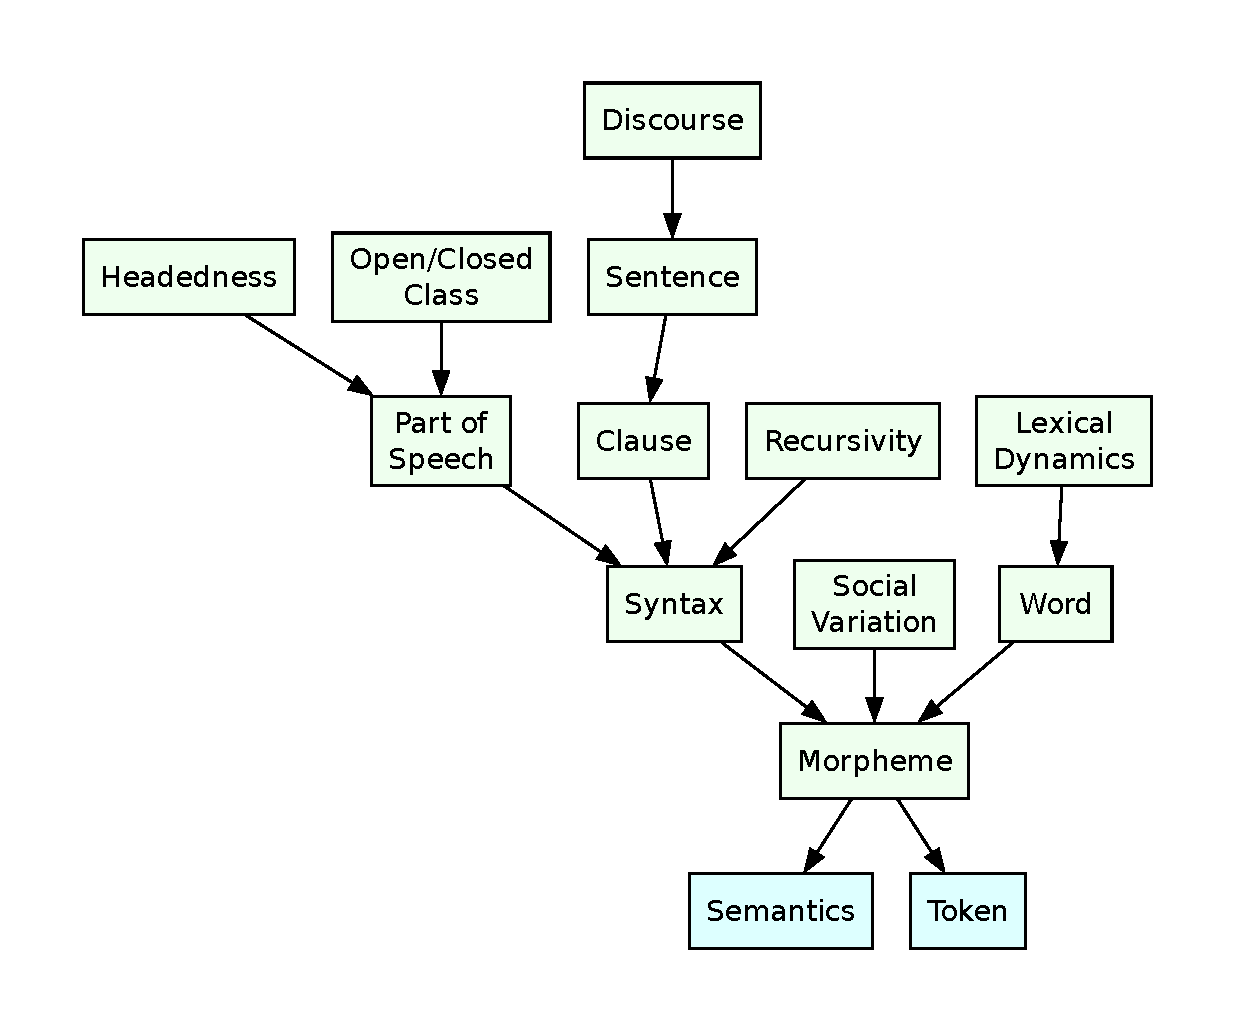
\includegraphics[width=0.95\linewidth]{assets/linguistic-dag}
  \caption{%
    Hierarchy of linguistic concepts.
    $X\rightarrow Y$ can be read as ``the definition of $X$ presupposes $Y$ being defined'' or roughly ``$X$ depends on $Y$''.
    The only concepts whose existence is established in emergent language are \emph{semantics} and \emph{token}.}
  \unskip\label{fig:linguistic-dag}
\end{figure}

In fact, there is a complex hierarchy of dependence of the various structures from across linguistics.
We illustrate hierarchy of some of the most fundamental linguistic structures in \Cref{fig:linguistic-dag}, representing the hierarchy as a transitively reduced directed acyclic graph.
At the bottom, we have foundational concepts like \emph{token} and \emph{semantics} while at the top we have concepts like \emph{headedness} and \emph{discourse}.
In the case of emergent languages, we can be sure of the existence of \emph{semantics} and \emph{tokens} and not much else.
Looking at the hierarchy, then, it would be necessary to establish the existence of \emph{morphemes} before being able to investigate phenomena like \emph{syntax} or \emph{parts of speech} in emergent communication.

\cmt{Necessary to establish the existence of, identify, define (specify, distinguish these).}

\cmt{Justify why we focus on structural characteristics?}


% \cmt{%
% Let's assume for a minute that one of the universals that we will need to detect is syntax.
% What we will need to do is create a definition of syntax in some generative sense: a language has syntax if its strings can be generated by such and such a process.
% (Is there are a more ``discriminative'' take on this process?)
% We'll need this generative take because we'll need to generate synthetic data that we can test our ``discriminative'' algorithm on given only surface forms (or surface forms + semantics).
% In addition to this generative definition, we'll need to introduce ideas of fuzziness either through non-strict adherence to the rules or by rules which inherently have some fuzz in them.
% Thus, we will have a definition of syntax which is applicable to EL since it doesn't make structural assumptions about human language as well as a process to generate synthetic data with varying levels/complexities/adherences to syntax which can for the basis of our detection algorithm.
% The idea here is that these synthetic languages will---by definition---show the full range of grammars (not necessarily very possible grammar).
% On the one hand, this feels like a bad approach because of course we can't cover every sense of grammar, but it seems like the most rigorous we can get.
% Maybe instead of saying ``we're testing for syntax full-stop'' we can say we are testing for ``$\alpha$-syntax'' which we define as being such and such: it isn't fully syntax but it is a reduced version that is easier to get to, setting a lower bar for emergent languages.
% \unskip}

Thus, this chapter will introduce an automated method for determining the presence and nature of morphemes in emergent language.
Additionally, it will also introduce a minimal definition of a syntax as proof-of-concept for identifying higher-level structures in emergent language.
These two concepts/structures are fundamental to defining and identifying other interesting features about language and so are prime candidates for foundational work in this research program.
In particular, this chapter will contribute the following items:
\begin{enumerate}[nosep]
  \item A definition of what morphemes are in the emergent languages, if they exist at all.
  \item An algorithm for determining the presence and identify of morphemes according to this definition.
  \item A minimal definition and extraction algorithm of syntax as a proof-of-concept extension of morpheme detection.
\end{enumerate}


\paragraph{Related Work}


\paragraph{Linguistics}
\cmt{URIEL \& lang2vec.}
\cmt{Compare and contrast with the ``typical'' universals which don't apply to what we have at all.}

Based on Greenberg (the whole book), there are many different kinds of universals about human language, including ones concerning:
\begin{itemize}[nosep]
  \item Presence of structures, simpliciter (the kind this chapter focuses on)
  \item Particular syntactic features; e.g., VSO \textrightarrow{} prepositional
  \item ``Design features'' of language; e.g., displaced, learnable, generalizable, evanescent
  \item Diachronic phenomena
  \item Semantics
  \item Psycholinguistics
  \item Phonology
\end{itemize}



\paragraph{Emergent communication}

\cmt{HAS paper}
\cmt{grammar induction}
\cmt{categorial grammar for compositionality}



